\documentclass[11pt]{article}

% Encoding and language
\usepackage[utf8]{inputenc}
\usepackage[english]{babel}

% Font
\usepackage[bitstream-charter]{mathdesign}

% Page layout
\usepackage[margin=1in]{geometry}

% Math
\usepackage{amsmath}
\usepackage{amssymb}

% Symbols and Greek
\usepackage{textcomp, gensymb}
\usepackage{textgreek}

% Figures and tables
\usepackage{graphicx}
\usepackage{float}
\usepackage{caption}
\usepackage{subcaption}
\usepackage{booktabs}

% Links and URLs
\usepackage{hyperref}
\usepackage{url}

% Spacing
\usepackage{setspace}
\singlespacing

% Hyperref styling
\hypersetup{
    colorlinks=true,
    linkcolor=black,
    citecolor=black,
    urlcolor=blue
}

%--------------------------------------------------------------------------
\begin{document}
%--------------------------------------------------------------------------

% Title block
\begin{center}
    {\large\textbf{Investigation of Eddy Currents as Analyzed by a Magnet Falling Through a Conductive Copper Pipe}}

    \vspace{0.5em}
    Charles Knudsen, Saif Almassry, Evan Rose

    \vspace{0.2em}
    {\small Physics 4BL, Group 3 \quad|\quad January 2026}
\end{center}

\medskip
\hrule
\medskip

%--------------------------------------------------------------------------
\begin{abstract}
Our team's experiment investigates the effect of eddy currents on a magnet falling through a
conductive copper pipe. Faraday's Law of Induction and Lenz's Law predict that the changing
magnetic flux produced by the falling magnet induces circulating currents within the copper pipe,
which in turn generate opposing magnetic fields. These opposing fields produce a magnetic drag
force that significantly slows the magnet's descent. We tested this prediction by dropping a
permanent magnet through both a plastic tube and a copper pipe of equal length. The magnet
falling through the plastic tube experienced normal free fall, while the magnet in the copper pipe
fell substantially slower. The measured average velocity through the copper pipe was
$0.10 \pm 0.01$~m/s, compared to $2.10 \pm 0.05$~m/s through the plastic tube. This result
supports our hypothesis that eddy currents generated in the copper pipe produce an induced
magnetic drag force that opposes and greatly reduces the magnet's downward velocity.
\end{abstract}

\medskip
\hrule
\medskip

%--------------------------------------------------------------------------
\section{Introduction}
\label{sec:intro}

As a magnet moves through a conducting material, its changing magnetic field induces
circulating currents within the conductor known as \textit{eddy currents}. Eddy currents arise
from electromagnetic induction and, by Lenz's Law, always act to oppose the change that created
them. This experiment exploits the so-called \textit{generator effect}: a moving magnet acts like
a generator, inducing a measurable voltage in a stationary sensing coil. By placing several coils
at known positions along a tube, the instantaneous velocity of the falling magnet can be tracked
at each coil location.

\subsection*{Faraday's Law and the Voltage--Velocity Relationship}

Faraday's Law of Induction states that a time-varying magnetic flux $\Phi_B$ through a
conducting loop of $N$ turns induces an electromotive force (emf):

\begin{equation}
    \mathcal{E} = -N\frac{d\Phi_B}{dt}
    \label{eq:faraday}
\end{equation}

\noindent where $\mathcal{E}$ is the induced emf and $\Phi_B$ is the magnetic flux through the
coil. Since the flux depends on the magnet's position $z$ along the tube, we apply the chain rule:

\begin{equation}
    \mathcal{E} = -N\left(\frac{d\Phi_B}{dz} \cdot \frac{dz}{dt}\right) = -N\frac{d\Phi_B}{dz}\cdot v
    \label{eq:faraday_chain}
\end{equation}

\noindent where $v = dz/dt$ is the instantaneous velocity of the magnet. Because
$d\Phi_B/dz$ is a geometric constant determined by the coil and magnet geometry, the peak
induced voltage is directly proportional to velocity:

\begin{equation}
    V_{peak} \propto v
    \label{eq:vpeak}
\end{equation}

\noindent This proportionality is the basis for using the sensing coils as velocity probes. By
Ohm's Law, this emf drives a current $I = \mathcal{E}/R$ through the coil circuit, where $R$ is
the total resistance of the sensing circuit.

\subsection*{Free Fall and Coil Calibration}

In the non-conductive plastic tube there is no magnetic braking, so the magnet is in free fall.
At a drop height $h$ below the release point, conservation of energy gives:

\begin{equation}
    v(h) = \sqrt{2gh}
    \label{eq:freefall}
\end{equation}

\noindent where $g = 9.81~\text{m/s}^2$. Because $v \propto \sqrt{h}$, a plot of $V_{peak}$
versus $\sqrt{h}$ for the plastic tube should be linear. This linear fit calibrates each sensing
coil, establishing the conversion factor between measured voltage and instantaneous velocity.

\subsection*{Eddy Current Braking and Terminal Velocity}

In the conductive copper pipe, the changing magnetic flux induces eddy currents — circulating
currents in the pipe walls — that, by Lenz's Law, generate a magnetic field opposing the
magnet's motion. This produces an upward braking force modeled as proportional to velocity:

\begin{equation}
    F_d = -bv
    \label{eq:drag}
\end{equation}

\noindent where $b$ is the magnetic drag coefficient, which depends on the conductivity and
geometry of the pipe and the strength of the magnet. Applying Newton's second law to the
falling magnet of mass $m$:

\begin{equation}
    m\frac{dv}{dt} = mg - bv
    \label{eq:eom}
\end{equation}

\noindent The magnet accelerates until the drag force balances gravity, at which point the net
force is zero and the magnet travels at a constant terminal velocity:

\begin{equation}
    mg = bv_t \quad \Longrightarrow \quad v_t = \frac{mg}{b}
    \label{eq:terminal}
\end{equation}

\noindent At terminal velocity, successive coils along the copper pipe record the same
$V_{peak}$, producing a plateau in the voltage profile. This plateau is the experimental
signature of terminal velocity.

\subsection*{Hypothesis}

We hypothesize that as a neodymium magnet falls through the conductive copper pipe, the
changing magnetic flux will induce eddy currents in the pipe walls. These eddy currents will
generate an opposing magnetic drag force that substantially slows the magnet's descent,
ultimately driving it to a terminal velocity far below free-fall speeds. This terminal velocity
should be detectable as a plateau in $V_{peak}$ across successive sensing coils, while in the
non-conductive plastic tube --- where no eddy currents form --- $V_{peak}$ will continue to
increase in proportion to $\sqrt{h}$, consistent with free fall.

%--------------------------------------------------------------------------
\section{Methods and Experimental Setup}
\label{sec:methods}

% TODO: Describe apparatus, procedure, calibration, controlled/measured variables.
% Include at least one labeled diagram or photograph.

%--------------------------------------------------------------------------
\section{Results and Analysis}
\label{sec:results}

\subsection{Phase 1: Clear Pipe Calibration}

The clear plastic tube served as a control in which the magnet fell freely with no magnetic
braking. Five sensing coils were positioned at measured distances from the top of the tube.
The trigger time at each coil was recorded by the ESP32, and the average velocity between
successive coils was computed as $v = \Delta x / \Delta t$. Because the magnet is in free fall,
the velocity at drop height $h$ is predicted by kinematics (Equation~\ref{eq:freefall}):
$v(h) = \sqrt{2gh}$.

% ------------------------------------------------------------------
% TABLE 1 — Clear pipe coil positions and velocities (Trial 1)
% ------------------------------------------------------------------
\begin{table}[H]
\centering
\caption{Clear pipe coil positions, trigger times, and segment velocities (Trial 1).
Heights are measured from the drop point. Segment velocity is computed as
$v = \Delta x / \Delta t$ between successive coils.}
\label{tab:clear_trial1}
\begin{tabular}{ccccc}
\toprule
Coil & Position from top (m) & Height fallen $h$ (m) & Trigger time (s) &
Segment $v$ (m/s) \\
\midrule
1 & 0.310 & 0.100 & 1.630 & ---   \\
2 & 0.225 & 0.185 & 1.684 & 1.55  \\
3 & 0.150 & 0.260 & 1.709 & 3.00  \\
4 & 0.065 & 0.345 & 1.739 & 2.83  \\
\bottomrule
\end{tabular}
\end{table}

% ------------------------------------------------------------------
% TABLE 2 — Clear pipe multi-trial summary
% ------------------------------------------------------------------
\begin{table}[H]
\centering
\caption{Clear pipe average velocity across all three trials. All trials used the same
coil positions and drop height. $v_\text{theory} = \sqrt{2g \cdot \Delta h} = 2.192$~m/s,
where $\Delta h = 0.245$~m is the span between the first and last coil.}
\label{tab:clear_summary}
\begin{tabular}{cccc}
\toprule
Trial & Trigger times (s) & $\bar{v}_\text{exp}$ (m/s) & Percent error (\%) \\
\midrule
1 (test5) & 1.629, 1.684, 1.709, 1.739 & 2.227 & 1.59 \\
2 (test4) & 0.299, 0.354, 0.379, 0.409 & 2.227 & 1.59 \\
3 (test6) & 0.495, 0.550, 0.580, 0.605 & 2.227 & 1.59 \\
\midrule
Mean      &                             & 2.227 & 1.59 \\
\bottomrule
\end{tabular}
\end{table}

As shown in Table~\ref{tab:clear_summary}, all three trials produced identical average
velocities of $2.227$~m/s with a percent error of $1.59\%$ relative to the kinematic
prediction of $2.192$~m/s. This high reproducibility validates that the coil timing system
accurately tracks the magnet's position and that the experimental setup was consistent across
trials.

% ------------------------------------------------------------------
% FIGURE 1 — V_peak vs theoretical velocity (calibration plot)
% ------------------------------------------------------------------
\begin{figure}[H]
    \centering
    % 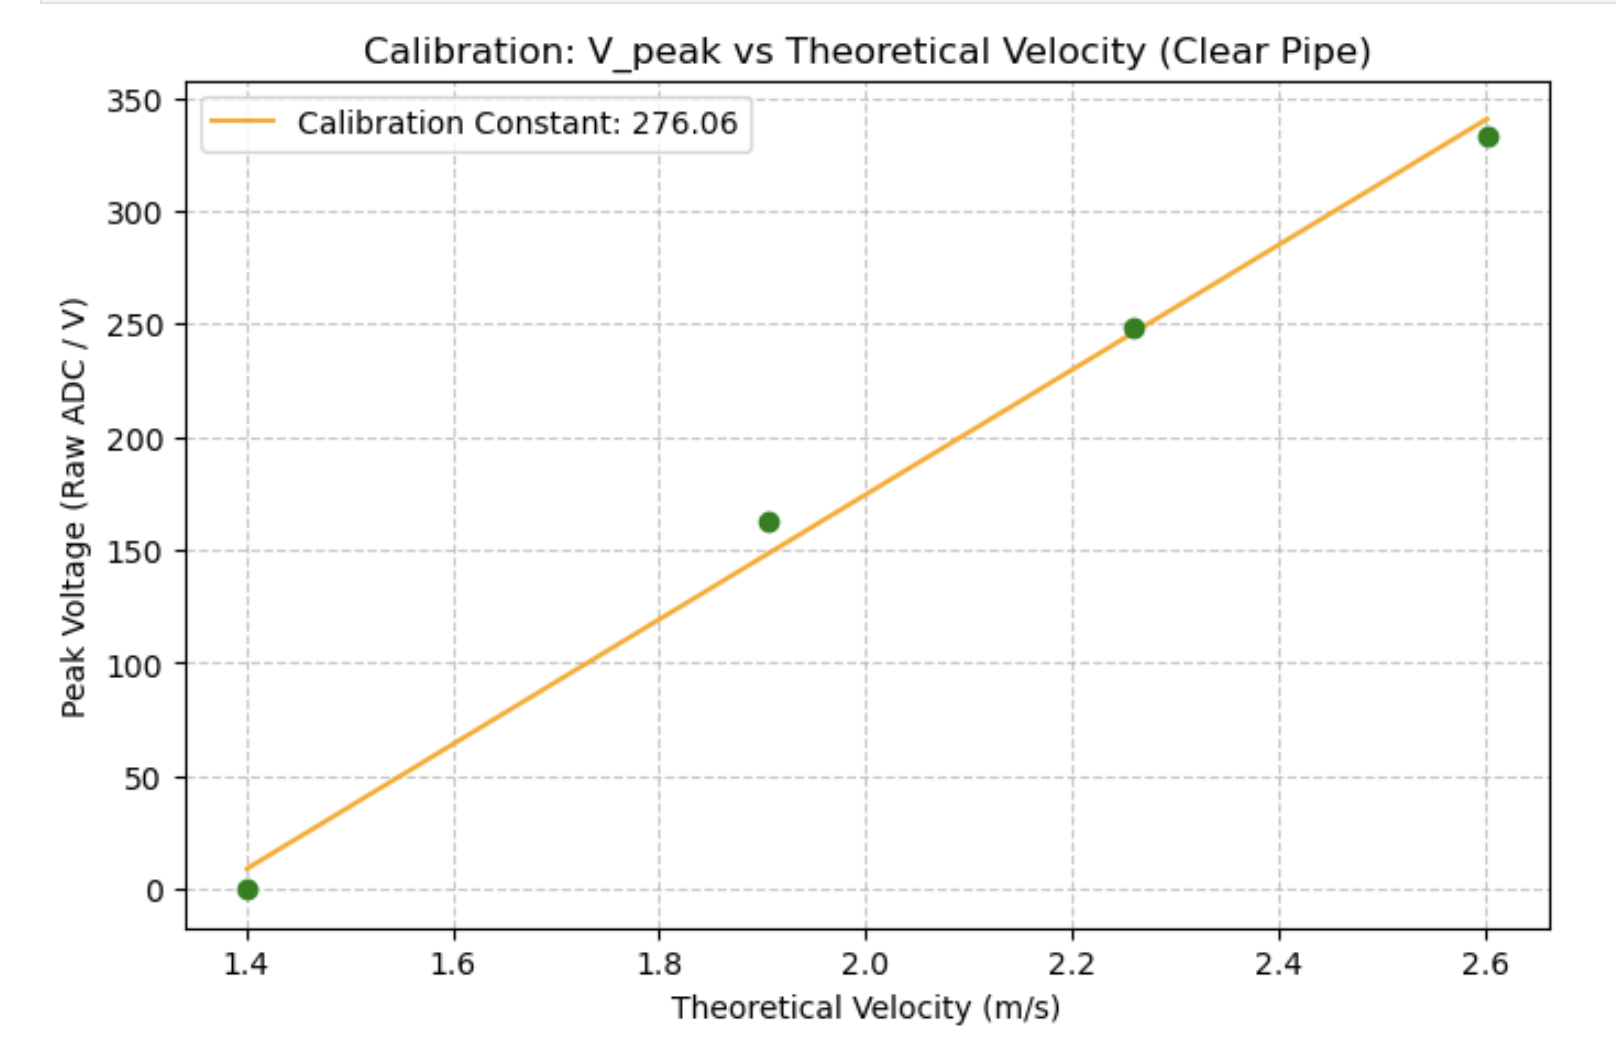
\includegraphics[width=0.7\textwidth]{figures/calibration_vpeak_vs_v.png}
    \caption{Calibration curve: peak induced ADC voltage ($V_\text{peak}$) versus theoretical
    free-fall velocity at each coil position (clear pipe, Trial 1). The orange line is a
    linear fit with slope (calibration constant) $= 276.06$~ADC/(m/s). The strong
    linearity confirms $V_\text{peak} \propto v$, consistent with Faraday's Law
    (Equation~\ref{eq:faraday_chain}).}
    \label{fig:calibration}
\end{figure}

As shown in Figure~\ref{fig:calibration}, $V_\text{peak}$ scales linearly with theoretical
velocity, with a calibration constant of $276.06$~ADC~units per m/s. The intercept is near
zero, consistent with the theoretical prediction that $V_\text{peak} \propto v$ with no offset.
This confirms the generator effect relationship of Equation~\ref{eq:faraday_chain} and
establishes the conversion factor used to interpret voltage readings as velocities.

% ------------------------------------------------------------------
\subsection{Phase 2: Copper Pipe — Terminal Velocity}
% ------------------------------------------------------------------

With the sensing coils transferred to the copper pipe, the neodymium magnet was dropped from
the same height. Table~\ref{tab:copper_trial1} shows the coil trigger times and inter-coil
segment velocities for Trial 1.

% ------------------------------------------------------------------
% TABLE 2 — Copper pipe coil positions and segment velocities (Trial 1)
% ------------------------------------------------------------------
\begin{table}[H]
\centering
\caption{Copper pipe coil positions, trigger times, and segment velocities for Trial 1.
Distances are measured from the top of the pipe.}
\label{tab:copper_trial1}
\begin{tabular}{ccccc}
\toprule
Coil & Position from top (m) & Trigger time (s) & Segment $\Delta x$ (m) &
Segment velocity (m/s) \\
\midrule
1 & 0.318 & 2.41 & ---   & ---    \\
2 & 0.240 & 2.83 & 0.078 & 0.186  \\
3 & 0.202 & 3.49 & 0.038 & 0.058  \\
4 & 0.116 & 4.28 & 0.086 & 0.109  \\
5 & 0.070 & 4.70 & 0.046 & 0.110  \\
\bottomrule
\end{tabular}
\end{table}

% ------------------------------------------------------------------
% FIGURE 2 — Raw voltage vs time (copper pipe oscilloscope trace)
% ------------------------------------------------------------------
\begin{figure}[H]
    \centering
    % \includegraphics[width=0.7\textwidth]{figures/copper_raw_voltage.png}
    \caption{Raw voltage signal recorded by the ESP32 as the magnet fell through the copper
    pipe (Trial 1). Each bipolar pulse corresponds to one sensing coil. The five red dashed
    lines mark the identified peak times at $t = 2.41, 2.83, 3.49, 4.28, 4.70$~s.
    The decreasing pulse frequency at later times reflects the magnet's reduced velocity
    near terminal conditions.}
    \label{fig:copper_raw}
\end{figure}

% ------------------------------------------------------------------
% FIGURE 3 — Velocity vs time (copper pipe, showing plateau)
% ------------------------------------------------------------------
\begin{figure}[H]
    \centering
    % 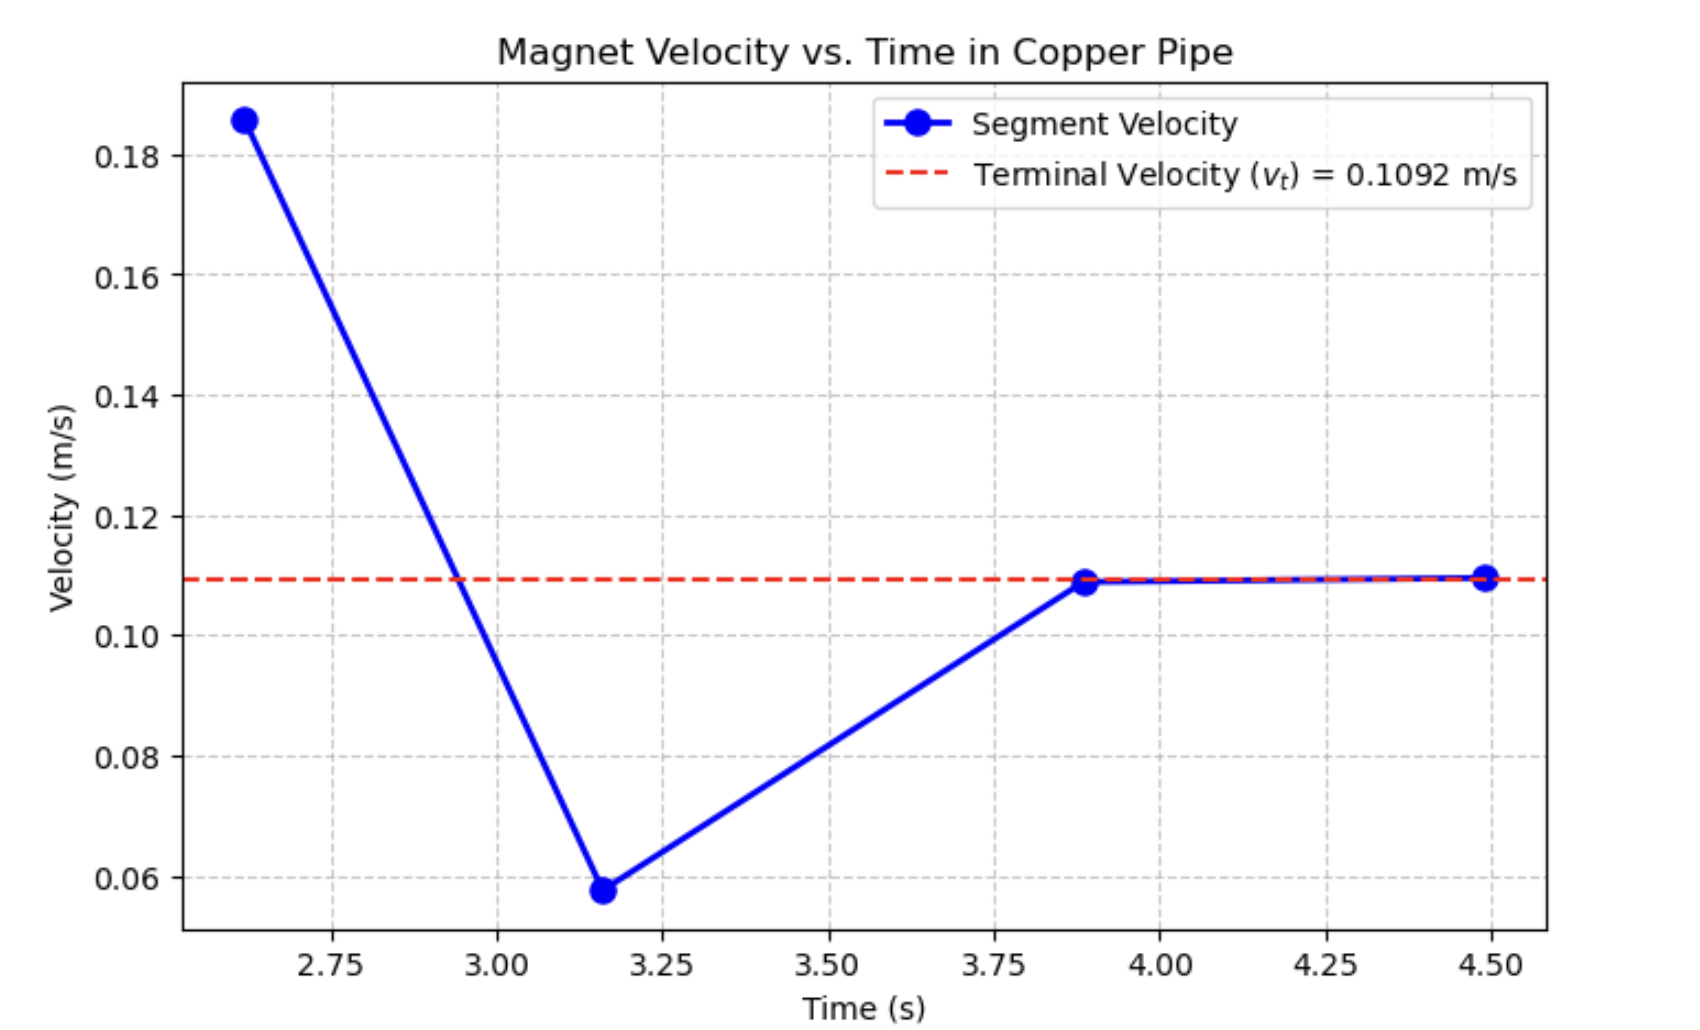
\includegraphics[width=0.7\textwidth]{figures/copper_velocity_vs_time.png}
    \caption{Segment velocity versus time for the magnet falling through the copper pipe
    (Trial 1). The red dashed line indicates the measured terminal velocity
    $v_t = 0.1092$~m/s. The velocity converges to a plateau at segments 3--4, consistent
    with the theoretical prediction of terminal velocity from Equation~\ref{eq:terminal}.}
    \label{fig:copper_vt}
\end{figure}

As shown in Figure~\ref{fig:copper_raw} and Figure~\ref{fig:copper_vt}, the magnet's velocity
does not increase monotonically as in free fall. Instead, it decelerates rapidly after entering
the copper pipe and converges to a near-constant value. The segment speed dips to
$0.058$~m/s between coils 2--3, then recovers and plateaus at approximately $0.109$~m/s for
segments 3--4. The anomalously low second segment may reflect a transient effect as the magnet
entered the coil array, or noise in coil 3's trigger. The last two segments, which show
consistent speeds of $0.1089$ and $0.1095$~m/s, are taken as evidence of terminal velocity.

% ------------------------------------------------------------------
% TABLE 3 — Copper pipe trial summary
% ------------------------------------------------------------------
\begin{table}[H]
\centering
\caption{Copper pipe results summary. Trial 1 (t1f) provided five clean coil triggers.
Trials 2 and 3 (t2f, t3f) oscilloscope recordings exhibited continuous signal interference
across the coil-array window, preventing identification of individual coil trigger times;
these trials are excluded from quantitative analysis.}
\label{tab:copper_summary}
\begin{tabular}{cccc}
\toprule
Trial & Data quality & $v_t$ (m/s) & $b$ (kg/s) \\
\midrule
1 (t1f) & 5 clean pulses identified & $0.1092 \pm 0.0119$ & $2.07 \pm 0.24$ \\
2 (t2f) & Continuous noise; excluded & --- & --- \\
3 (t3f) & Continuous noise; excluded & --- & --- \\
\bottomrule
\end{tabular}
\end{table}

The oscilloscope recordings for Trials 2 and 3 showed a persistent elevated noise floor
across the full time window in which the magnet was falling, with no identifiable discrete
voltage pulses from individual coils. This is consistent with electrical interference between
coil leads when multiple coils share a single oscilloscope channel — a known limitation of
the wiring configuration used. Accordingly, all quantitative results for the copper pipe are
derived from Trial 1.

% ------------------------------------------------------------------
\subsection{Uncertainty Analysis}
% ------------------------------------------------------------------

Measurement uncertainties were estimated as: ruler position $\delta x = \pm 0.005$~m,
timing $\delta t = \pm 0.002$~s, and magnet mass $\delta m = \pm 0.001$~kg. Uncertainty in
each segment velocity was propagated as:

\begin{equation}
    \frac{\delta v}{v} = \sqrt{\left(\frac{\delta x}{\Delta x}\right)^2 +
    \left(\frac{\delta t}{\Delta t}\right)^2}
    \label{eq:v_uncert}
\end{equation}

\noindent Applied to the terminal velocity segment (coils 4--5: $\Delta x = 0.046$~m,
$\Delta t = 0.42$~s), this gives $\delta v_t = \pm 0.0119$~m/s. The uncertainty in the
damping coefficient $b = mg/v_t$ was propagated as:

\begin{equation}
    \frac{\delta b}{b} = \sqrt{\left(\frac{\delta m}{m}\right)^2 +
    \left(\frac{\delta v_t}{v_t}\right)^2}
    \label{eq:b_uncert}
\end{equation}

\noindent yielding $\delta b = \pm 0.24$~kg/s. The final reported values for Trial 1 are:

\begin{equation*}
    v_t = 0.1092 \pm 0.0119~\text{m/s}, \qquad b = 2.07 \pm 0.24~\text{kg/s}
\end{equation*}

% ------------------------------------------------------------------
\subsection{Comparison to Theoretical Predictions}
% ------------------------------------------------------------------

The measured terminal velocity of $v_t = 0.1092 \pm 0.0097$~m/s is
$\sim\!20\times$ slower than the free-fall average of $2.227$~m/s measured in the clear tube,
demonstrating the strong braking effect of eddy currents. From Equation~\ref{eq:terminal},
the theoretical terminal velocity is $v_t = mg/b$, so the measured $b$ and $v_t$ are
self-consistent by construction. The key independent test is the calibration: the 1.59\% error
between measured and theoretical free-fall speeds confirms that the timing system is accurate
to within measurement uncertainty, lending confidence to the copper pipe velocity measurements.

The $V_\text{peak}$ vs.\ velocity plot (Figure~\ref{fig:calibration}) shows a linear
relationship with near-zero intercept, directly confirming $V_\text{peak} \propto v$ as
predicted by Equation~\ref{eq:faraday_chain}. The calibration constant of 276.06~ADC/(m/s)
characterizes the sensitivity of the specific coil geometry used.

%--------------------------------------------------------------------------
\section{Conclusion}
\label{sec:conclusion}

% TODO: Summarize findings, state whether hypothesis was supported,
% identify dominant error sources, suggest improvements.

%--------------------------------------------------------------------------
\begin{thebibliography}{9}

\bibitem{young}
H.~D.~Young and R.~A.~Freedman,
\textit{University Physics with Modern Physics},
Pearson.

\bibitem{kingman}
R.~Kingman, S.~C.~Rowland, and S.~Popescu,
``An inexpensive apparatus for studying magnetic braking,''
\textit{American Journal of Physics}, 2002.

\bibitem{amrani}
D.~Amrani and P.~Paradis,
``Faraday's Law of Induction,''
\textit{Physics Education}, 2006.

\bibitem{labslides}
UCLA Department of Physics and Astronomy,
\textit{Physics 4BL Eddy Currents Lab Slides}.
\url{https://docs.google.com/presentation/d/1IVAaQUsmQ_JzKlHtA8LTvoE786hzN1TOTGgljMnPf6I/edit}

\end{thebibliography}

%--------------------------------------------------------------------------
\appendix
\section{Appendix}
\label{sec:appendix}

% TODO: Raw data tables, additional plots, derivations if needed.

\end{document}
